\section{Results}

At the conclusion of Run 3, in December of 2013, a total of 10 Bq of tritium was injected into LUX and removed. A total 325,000 events were observed in the active volume of LUX, of which 183,000 events were in the fiducial volume at the nominal LUX electric field of 180 V/cm. Another 4,500 fiducial events were collected in a special run at a reduced field of 105 V/cm. We correct the S1 and S2 signals for spatial effects such as the light collection efficiency and the free electron lifetime with $\rm ^{83m}$Kr data as described in \cite{lux-reanalysis}. 


We interpret the data in terms of the combined energy model for electron recoils \cite{Platzman}, where the total energy of an event is directly proportional to the number of quanta produced (electrons plus scintillation photons):

\begin{equation}
\rm E_{total} = W \cdot (n_{\gamma} + n_e )
\label{platzman_eq}
\end{equation}

\noindent
where $\rm E_{total}$ is the energy of the deposition in keV and  $\rm n_\gamma$ and $\rm n_e$ are the number of photons and electrons respectively. We use a $W$ value of 13.7 $\rm \pm$ 0.2 eV/quanta \cite{Dahl_Thesis}. In LUX $n_{\gamma}$ and $n_e$ are proportional to the S1 and S2 signals, with gain factors $g_1$ and $g_2$: 
%We use a $W$ value of 13.7 $\rm \pm$ 0.2 eV/quanta \cite{Dahl_Thesis}. In LUX $n_{\gamma}$ and $n_e$ are proportional to the S1 and S2 signals, with gain factors $g_1$ and $g_2$:

\begin{equation}
\rm E_{total} = W \cdot \left(\frac{S1}{g_1} + \frac{S2}{g_2} \right)
\label{energy_eq}
\end{equation}

\noindent
where S1 and S2 have units of photons detected (phd) and $g_1$ and $g_2$ have units of phd per quanta. $g_1$ is the average light collection efficiency times the average quantum efficiency of the PMT arrays, while $g_2$ is the product of the electron extraction efficiency at the liquid-gas surface and the average single electron size in phd. $g_1$ and $g_2$ are measured with line source data in the LUX Run 3 to be $0.120 \pm 0.002$ and $10.63 \pm 0.015$ \cite{lux-reanalysis, lux-prd}. For the December 2013 tritium calibration presented here, the gains g1 and g2 are constrained by optimizing the combined energy model to the true tritium spectral shape \cite{Tritium_Eq_Simpson} convolved with detector resolution. We find values of $g_1$ = \gone  ~and  $g_2$ = \gtwo.  The difference between these values with those quoted in Ref. \cite{lux-reanalysis, lux-prd} is taken as a systematic error for the results present in Ref. \cite{lux-reanalysis, lux-prd}.

\begin{figure}[h!]\centering
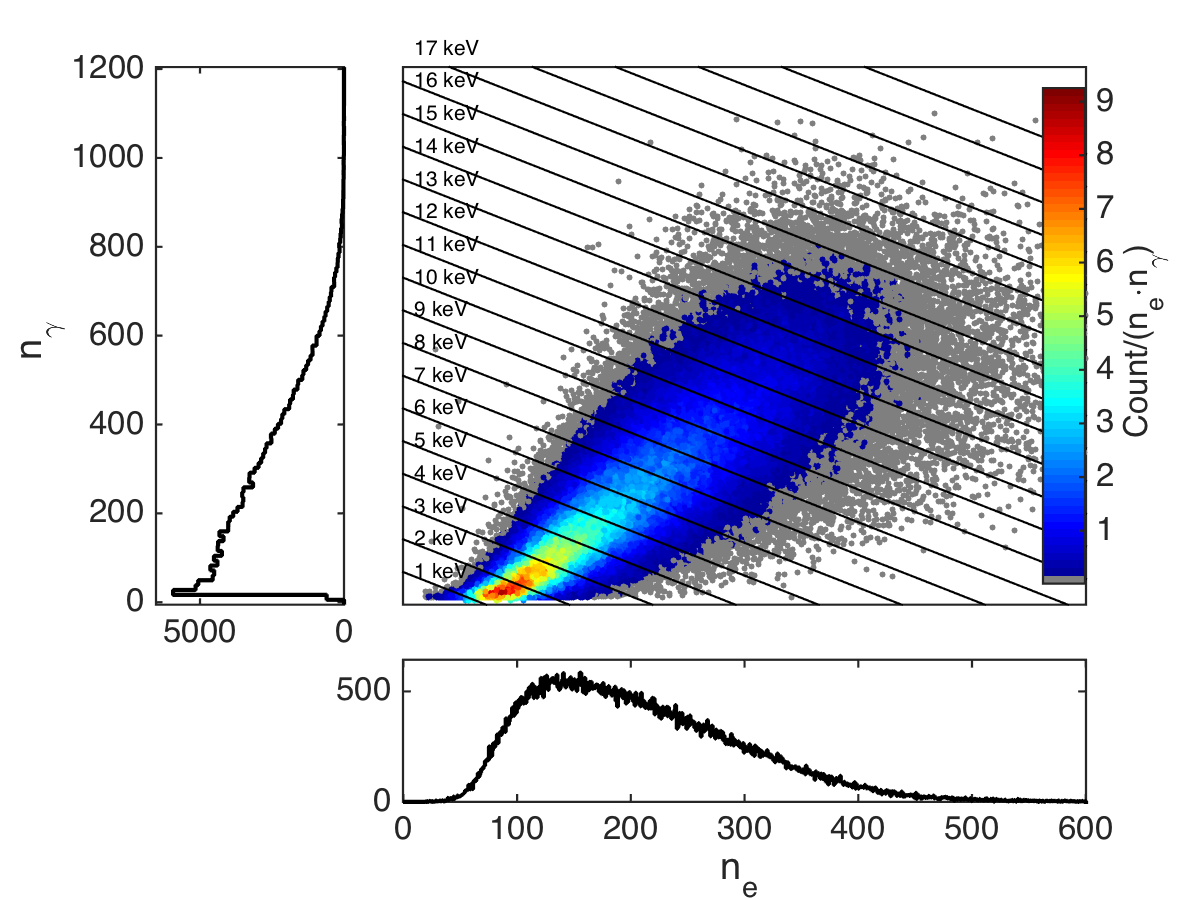
\includegraphics[width=90mm]{fig/tritium_scatter.png}
\caption{Scatter plot of $n_e$ vs $n_{\gamma}$ for 149,000 fiducial tritium events at 180 V/cm. Lines of constant energy are indicated assuming a $W$ value of 13.7 eV/quanta. The data is projected into $n_e$ and $n_{\gamma}$ histograms on each axis.}
\label{fig:tritium-scatter}
\end{figure}


\begin{figure}[h!]
\begin{center}
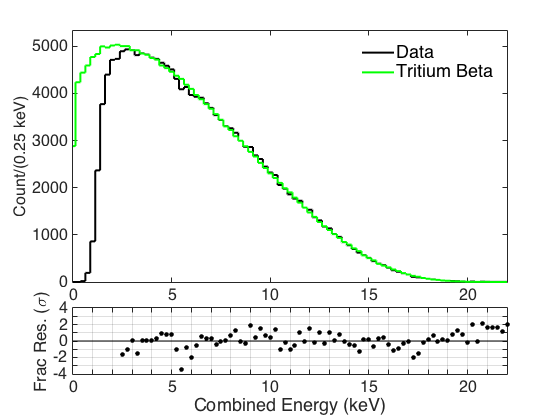
\includegraphics[width=90mm]{fig/tritium-spectrum-linear.png}
\caption{The tritium energy spectrum measured by LUX with the combined energy model (black) compared to several theory models: a pure tritium spectrum (dashed blue), and a tritium spectrum convolved with detector resolution  $\rm \frac{\sigma_E}{W} = \sqrt{\sigma^2(n_{\gamma})+ \sigma^2(n_e)}$. }
\label{fig:tritium-spectrum}
\end{center}
\end{figure}

%S1 ($\rm \sigma(n_{\gamma}))$ and S2 ($\rm \sigma(n_e)$)

A scatter plot of $n_e$ vs $n_{\gamma}$ for the tritium data at 180 V/cm is shown in Fig. \ref{fig:tritium-scatter}, along with the projected histograms on each axis. Contours of constant energy in 1 keV intervals are also plotted, derived from Eq. \ref{platzman_eq}. 


The tritium energy spectrum, obtained by projecting the data along the lines of constant energy, is shown in Fig. \ref{fig:tritium-spectrum}. The data are compared to an ideal tritium spectrum \cite{Tritium_Eq_Simpson}, with no detector effects, and a tritium spectrum with an energy smearing factor of $\rm \frac{\sigma_E}{W} = \sqrt{\sigma(n_{\gamma})^2 + \sigma(n_e)^2}$, where $\rm \sigma(n_{\gamma})$ and $\rm \sigma(n_e)$ represent the detector resolution for photon and electron counting. The ratio of the data to the smeared theoretical spectrum is shown in Fig. \ref{fig:ER-threshold}, along with an empirical fit to an error function. The effective 50\% energy threshold is found to be 1.30 $\pm$ 0.013 keV. The good agreement between data and theory from 2 keV to the endpoint of the tritium spectrum supports the combined energy model in Eq.\ref{platzman_eq}.

\begin{figure}[h!]\centering
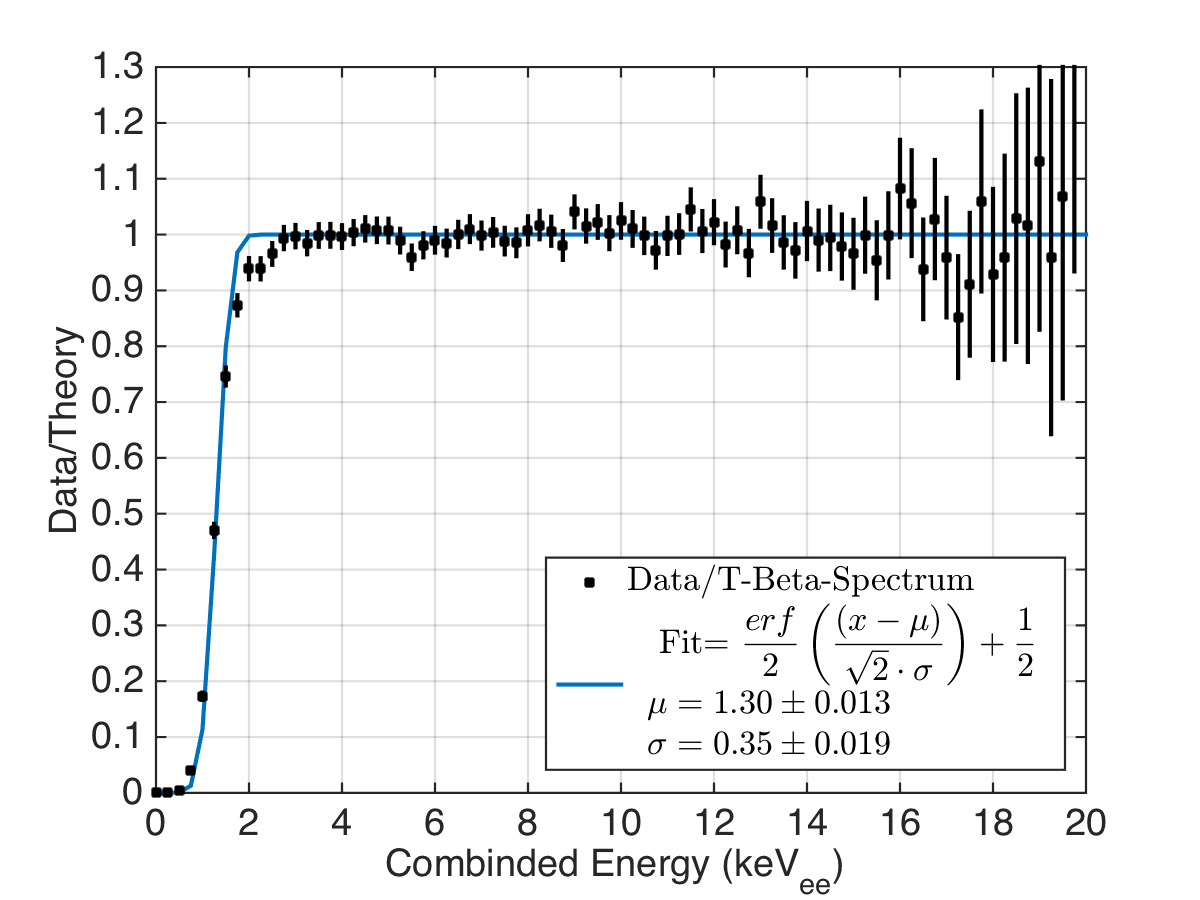
\includegraphics[width=90mm]{fig/E_Thres_Fit.png}
\caption{ER threshold measured by comparing the measured energy spectrum to the smeared tritium spectrum. A fit to an error function is shown.}
\label{fig:ER-threshold}
\end{figure}


%Individual events on the plot are smeared by detector resolution and electron-ion pair recombination fluctuations. Detector resolution is comprised of statistical fluctuations in counting photons and electrons in the S1 and S2 channel. The finite resolution in S1 and S2 smear events along the vertical and horizontal axis, respectively. Recombination fluctuations ($\rm \sigma(R)$) smear events along the contours of constant energy, and thus cancel out in the combined energy model of Eq.\ref{platzman_eq}. 


The mean light and charge yields of ER events in LUX are obtained by dividing the mean light and charge signals by the combined energy in each energy bin. The result is shown for 180 V/cm and 105 V/cm in Fig. \ref{fig:ER-LY-QY} along with NEST v0.98 model predictions at each field \cite{NEST_2013}. For these plots a small correction has been applied to the data to account for smearing of tritium events across energy bins due to the detector's resolution and the spectral shape \cite{Dobi_Thesis}\footnote{We have verified with an internal $^{83m}Kr$ calibration source that the light yield of LXe is unaffected by the presence of CH$_4$ at concentrations up to $\sim$1 part per million. For the CH$_3$T measurements reported here the concentration was ($<$ $\rm10\times10^{-12}$ g/g). }

\begin{figure}[h!]\centering
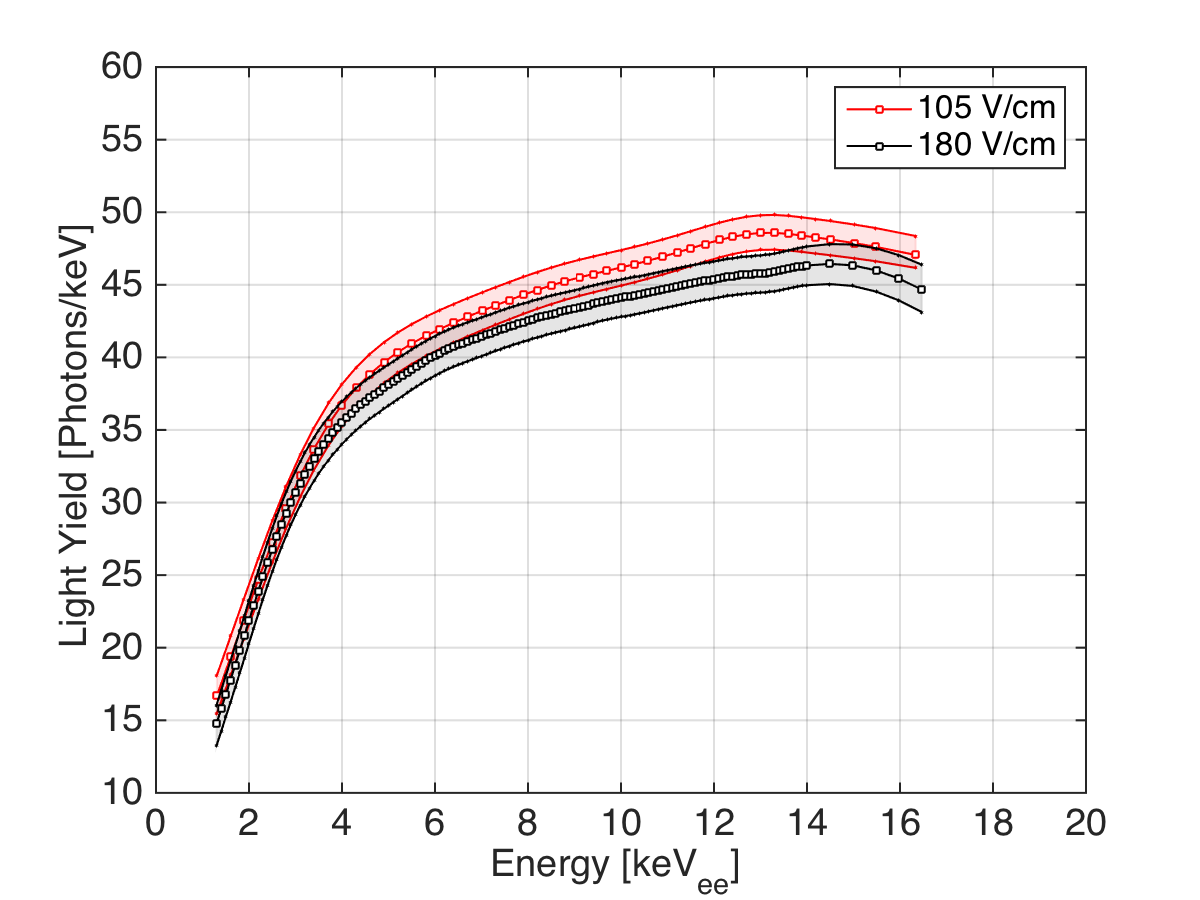
\includegraphics[width=90mm]{fig/ER_LY.png}
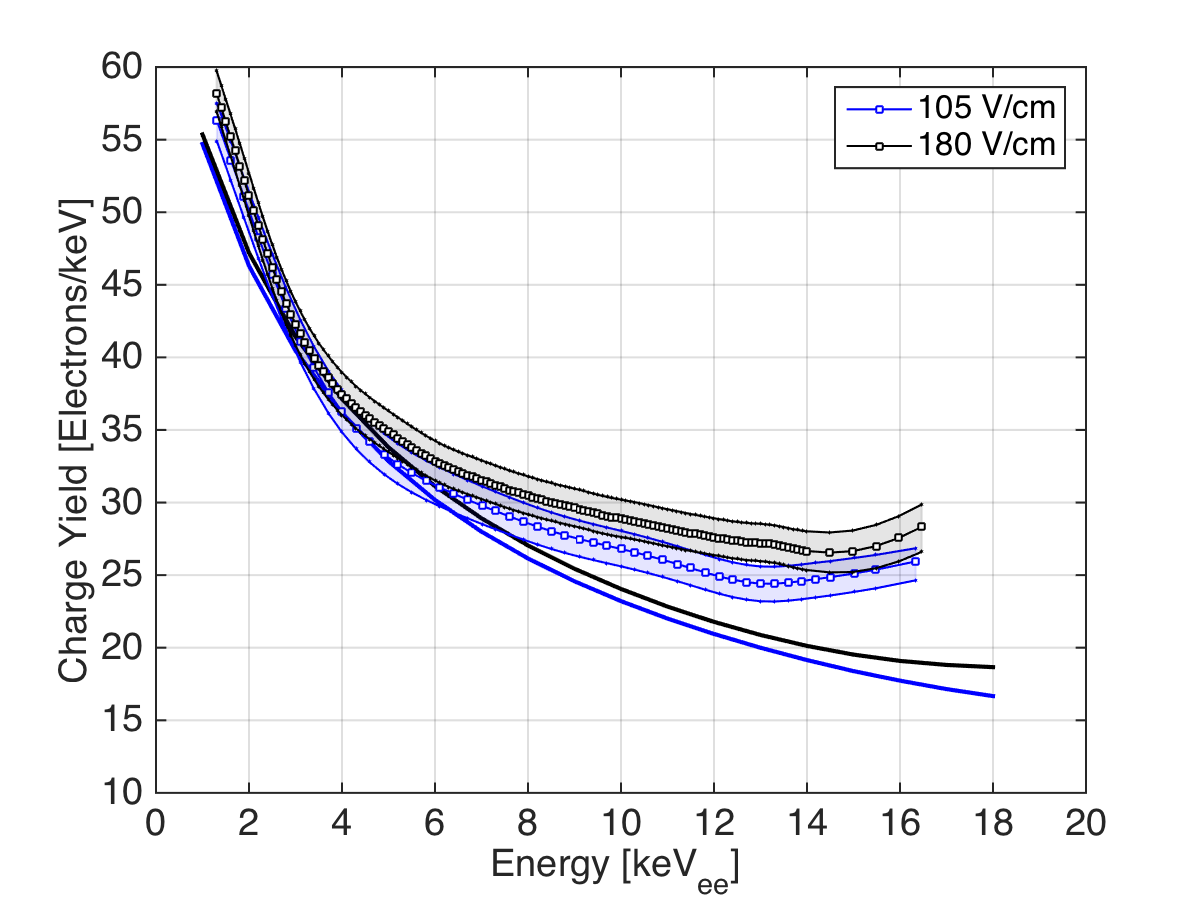
\includegraphics[width=90mm]{fig/ER_QY.png}
\caption{The light yield and charge yield of ER events in LUX at 180 V/cm (black) and 105 V/cm (blue) compared to NEST v0.98 (2013). The bands indicate the systematic errors on $g_1$ and $g_2$, which are fully correlated across all energy bins. $g_1$ is anti-correlated with $g_2$, such that an increase in the charge yield within the grey band must be compensated by an equivalent decrease in the light yield. Upper: Light yield. Lower: the charge yield. The solid lines represent the NEST model predictions at each field \cite{NEST_2013}.}
\label{fig:ER-LY-QY}
\end{figure}

The light yield measurements are compared to similar measurements by other authors in Fig. \ref{fig:Re_LY}. To remove detector effects from this comparison, the light yield is normalized to the yield of the 32.1 keV electron capture decay of $\rm ^{83m}Kr$ at zero electric field. For LUX this light yield is measured to be $\rm 63.8 \pm 3$ $\rm n_\gamma$/keV. The findings are consistent with the expectation that the tritium light yields at 105 and 180 V/cm lie between those at zero field and 450 V/cm from \cite{Aprile_LY} and \cite{Baudis}. It is worth noting that Refs. \cite{Aprile_LY} and \cite{Baudis} use Compton scatters as the source of ER events, while in tritium data the ER source is a beta decay. At low energy beta decays and Compton scatters should leave similar track lengths and produce similar event characteristics. The comparison of Fig. \ref{fig:Re_LY} confirms this expectation within the experimental uncertainties.

\begin{figure}[h!]\centering
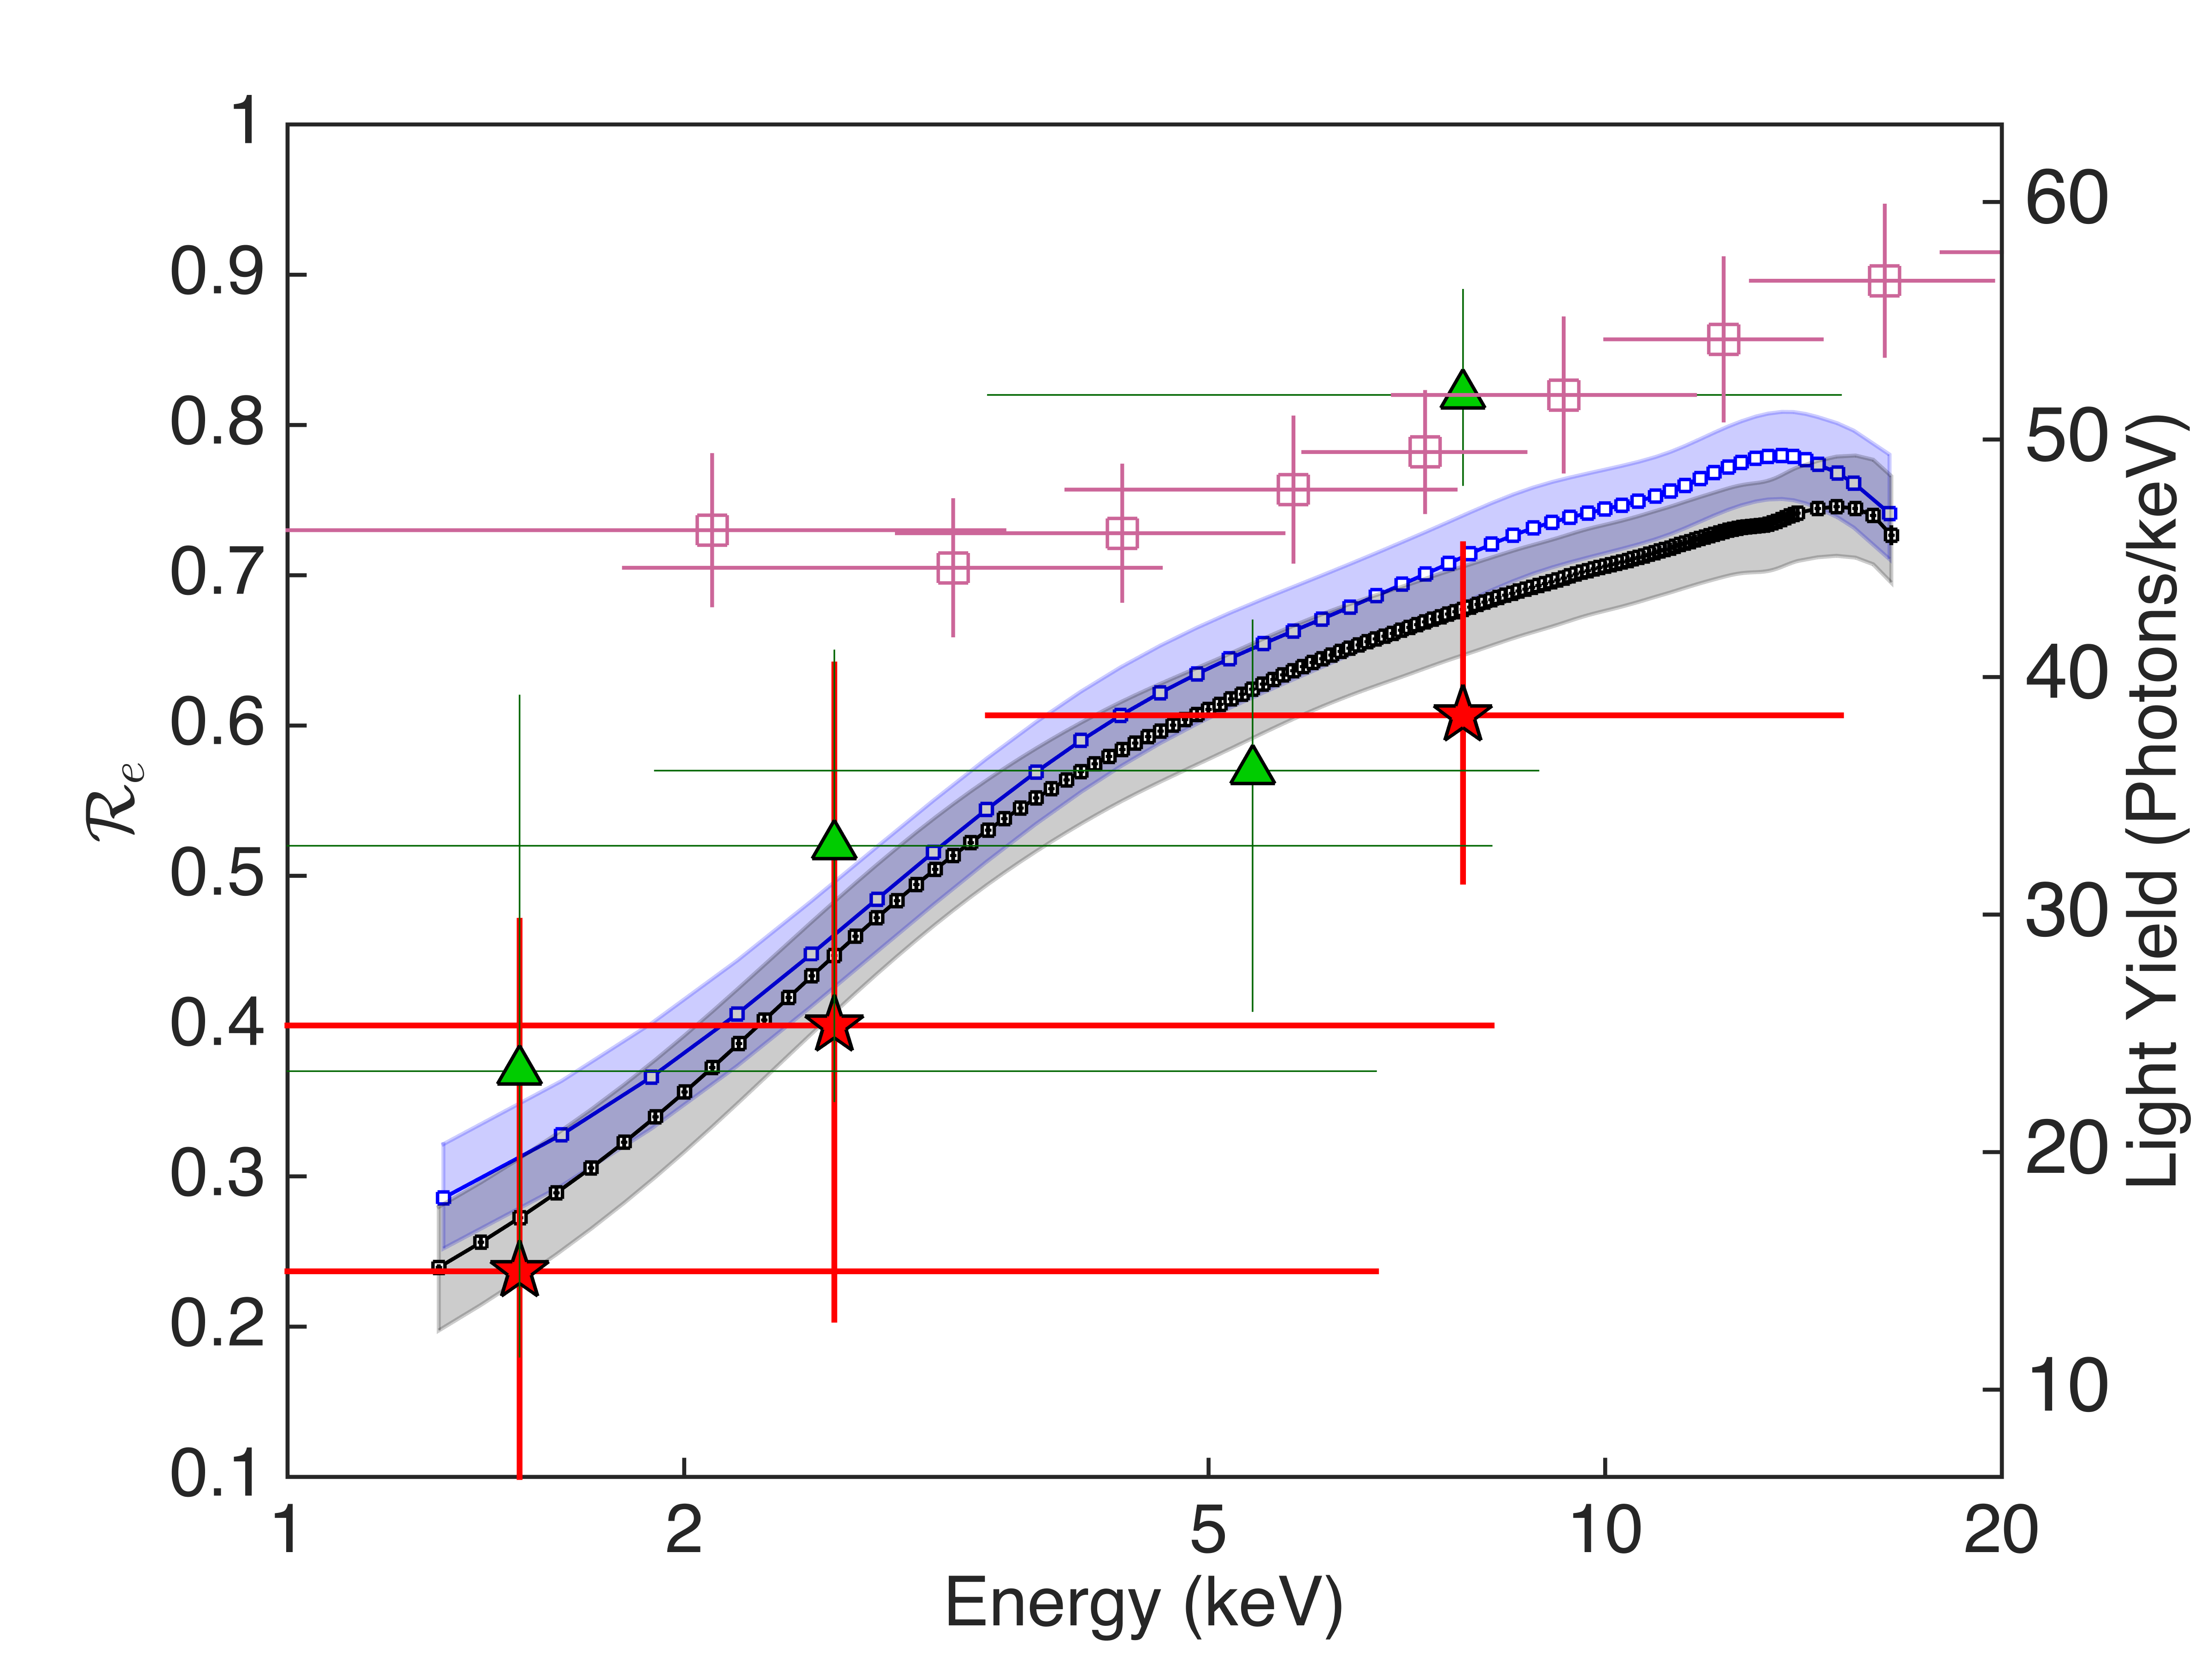
\includegraphics[width=88mm]{fig/Re_LY_log.png}
\caption{Light yield measurement from LUX tritium data compared to results from other authors. Left vertical scale: light yield relative to that of the 32.1 keV decay of $\rm^{83}Kr $ at zero field. Right vertical scale: absolute light yield measurements from LUX tritium data. Shaded blue curve is tritium at 105 [V/cm], shaded black curve is tritium at 180 [V/cm]. Magenta squares represent zero field measurements from \cite{Aprile_LY}. Cyan triangles and red circles represent a Compton scattering measurement at zero field and 450 [V/cm] from \cite{Baudis}. }
\label{fig:Re_LY}
\end{figure}


As shown in Fig. \ref{fig:ER-LY-QY}, we find that the light yield increases rapidly from 1 and 6 keV, and then becomes mostly energy independent over the remainder of the tritium spectrum. The charge yield exhibits the complimentary behavior as expected from the combined energy model. These effects can also be illustrated by plotting the number of photons and electrons as a function of energy, as shown in Fig. \ref{fig:quanta-vs-energy}. Also shown in Fig. \ref{fig:quanta-vs-energy} are the total number of quanta assuming a $W$ value of 13.7 eV/quanta (black), and the initial number of ions (violet) and excitons (cyan) prior to recombination, where we assume an exciton-to-ion ratio of 0.2 \cite{Doke_alpha} independent of energy. Under this assumption we interpret the charge yield data as a measure the recombination fraction at each energy according to

\begin{equation}
r = \frac{\frac{n_{\gamma}}{n_e} - \alpha}{\frac{n_{\gamma}}{n_e} + 1}
\end{equation}

\noindent
where $r$ is the recombination fraction and $\alpha$ is the initial exciton-to-ion ratio. The implied recombination fraction as a function of energy is shown in Fig. \ref{fig:recombination}. Here the falling charge yield and rising light yield between 1 and 6 keV appears as a rapid rise in the recombination fraction with increasing energy. 

\begin{figure}[h!]\centering
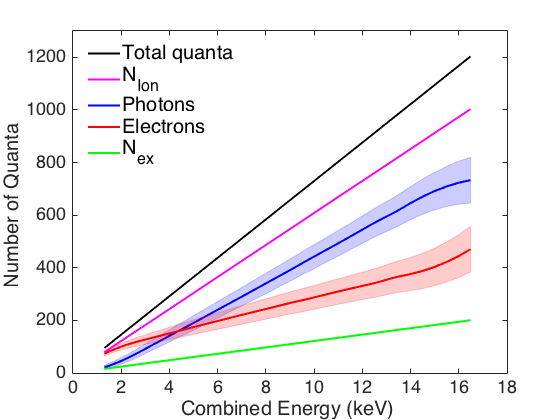
\includegraphics[width=90mm]{fig/quanta-vs-energy.png}
\caption{Top: The mean number of electrons (red) and scintillation photons (blue) produced in LUX at 180 V/cm as a function of energy. The bands indicate the correlated systematic errors on $g_1$ and $g_2$. Also shown are the total number of quanta, primary ions, and primary excitons, assuming an exciton to ion ratio of 0.2. }
\label{fig:quanta-vs-energy}
\end{figure}

\begin{figure}[h!]\centering
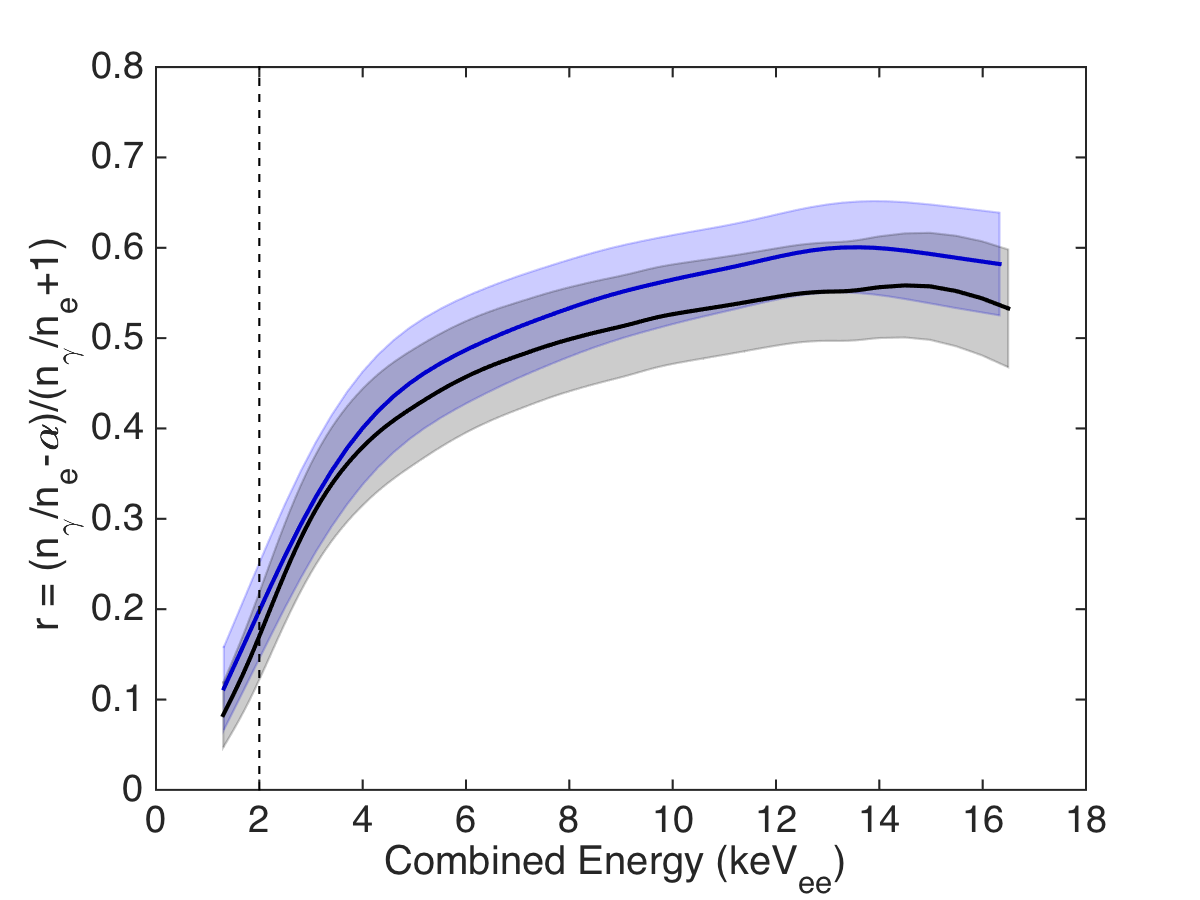
\includegraphics[width=90mm]{fig/recombination.png}
\caption{Recombination fraction of ER events at 180 V/cm (black) and 105 V/cm (blue), assuming an exciton-to-ion ratio of 0.2.}
\label{fig:recombination}
\end{figure}

\begin{figure}[h!]\centering
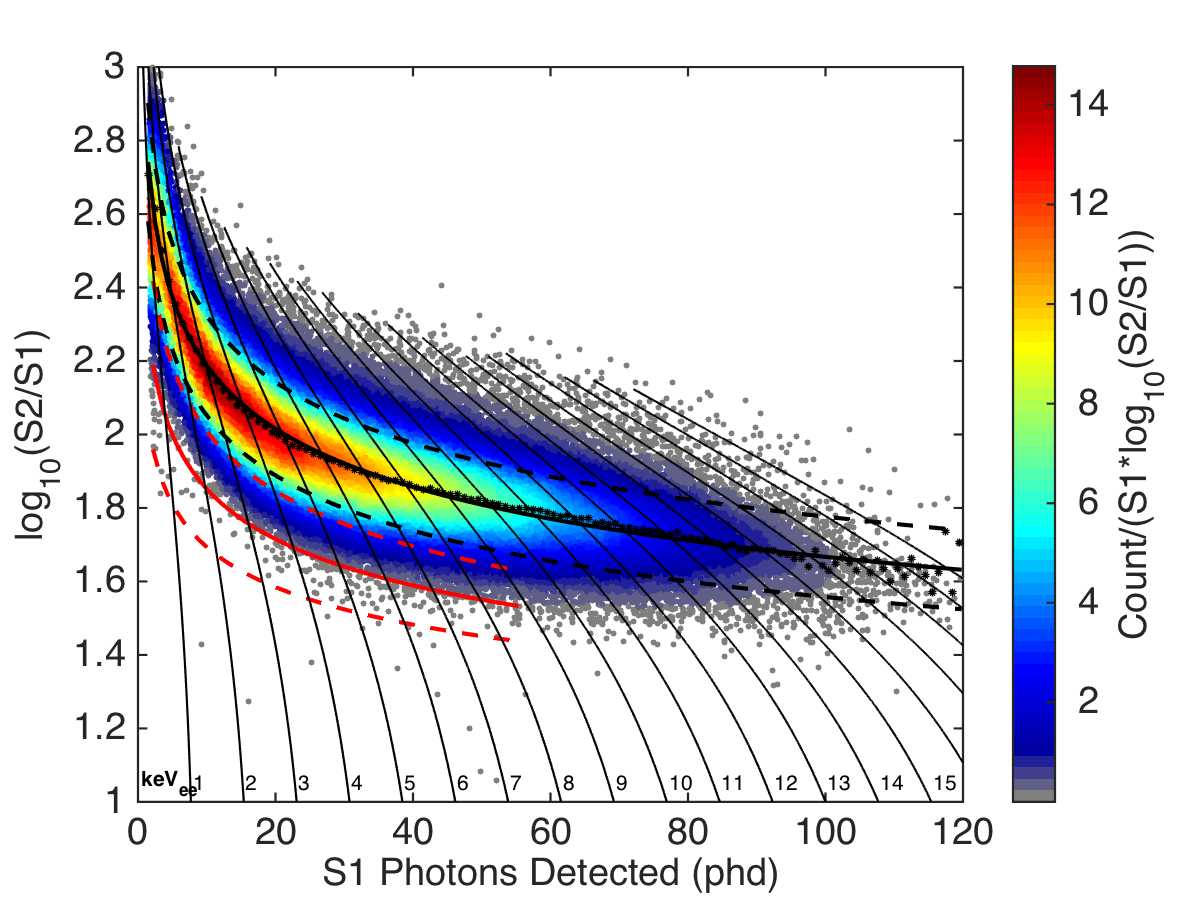
\includegraphics[width=90mm]{fig/CH3T_ER_Band.png}
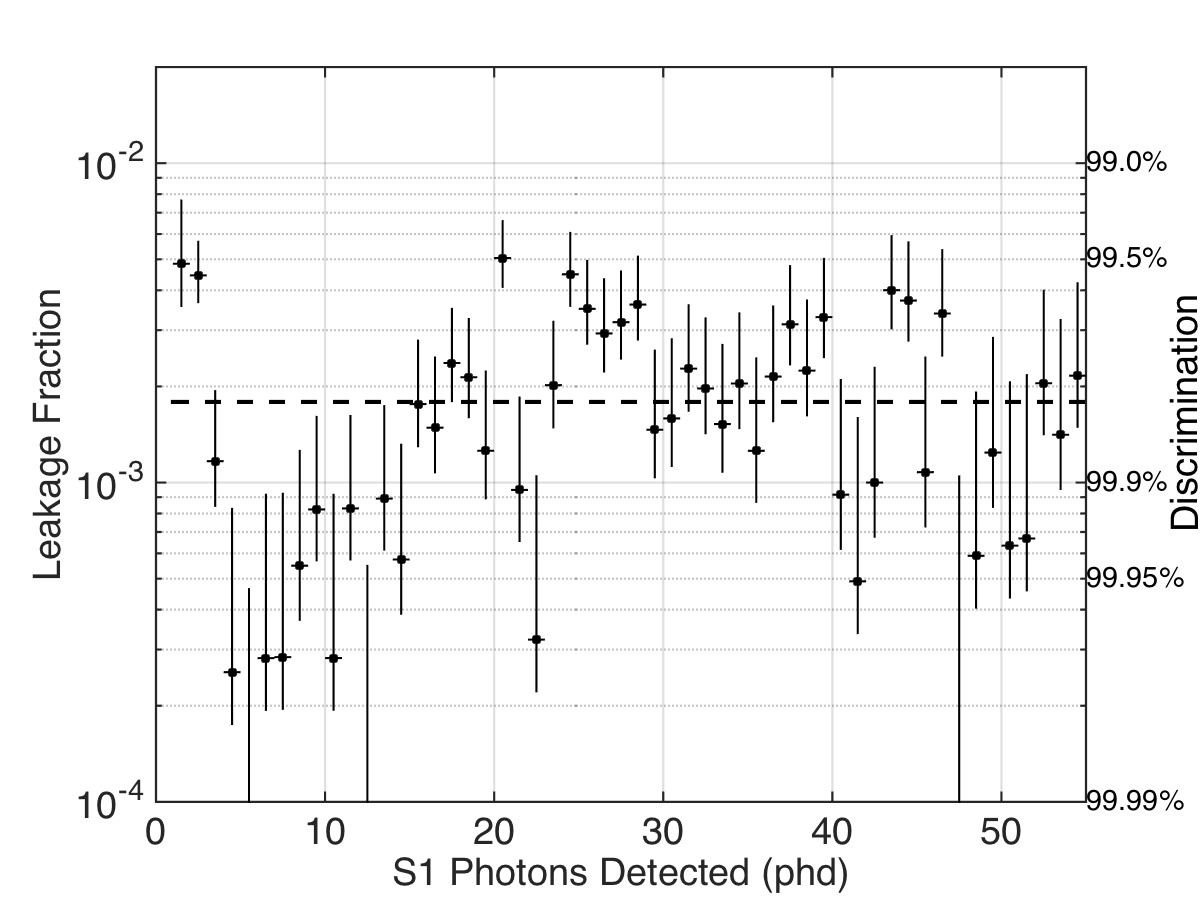
\includegraphics[width=85mm]{fig/CH3T_Leakage_Run03.png}
\caption{Top: The electron recoil band of LUX illuminated by 130,000 tritium events at the nominal LUX electric field of 180 V/cm.  The recoil discriminant variable, log(S2/S1), is shown vs. S1 between 1 and 120 phd in S1 (with contours of constant energy $\rm1-20 \, keV_{ee}$). Also indicated in black are the mean and the 10\% and 90\% contours of the ER population. The solid red line represents the mean NR band determined with DD neutron generator data. The dashed red indicates the 10\% and 90\% contours of the NR band. Bottom: LUX recoil discrimination vs. S1. Y-axis labels: left -  leakage fraction ($f$); right - discrimination ($1-f$).}
\label{fig:ER_band}
\end{figure}

%\begin{figure}[h!]\centering
%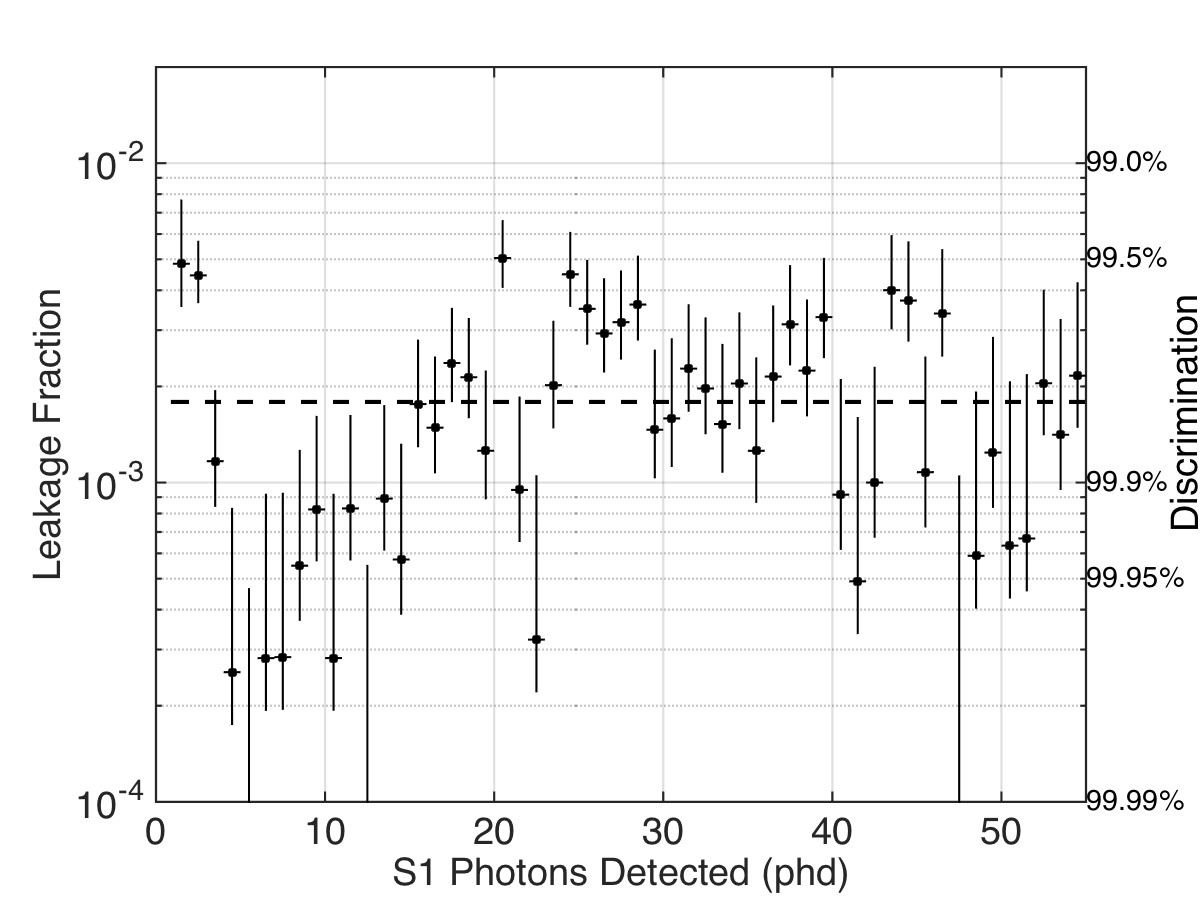
\includegraphics[width=90mm]{fig/CH3T_Leakage_Run03.png}
%\caption{LUX recoil discrimination vs. S1, determined from Fig. \ref{fig:ER_band}. Y-axis labels: left -  leakage fraction ($f$); right - discrimination ($1-f$).}
%\label{fig:Leak}
%\end{figure}



The LUX ER band is shown as log$_{10}$(S2/S1) vs S1 in Fig. \ref{fig:ER_band}(top).  Also shown is the LUX NR band measured with neutron generator data\cite{DD-paper, lux-reanalysis}. The ER band has a characteristic rise at decreasing values of S1 which reflects the increasing charge yield and decreasing light yield below $\sim$6 keVee. The leakage fraction ($f$), defined as the fraction of ER events that fall below the mean of the NR band, is shown in Fig. \ref{fig:ER_band}(bottom) as a function of S1. The recoil discrimination ($1-f$) has an average value of \fixit{99.8\%} for events with S1 between 1 and 50 phd.


\onecolumngrid
\break
\begin{sidewaysfigure}[p!]\centering
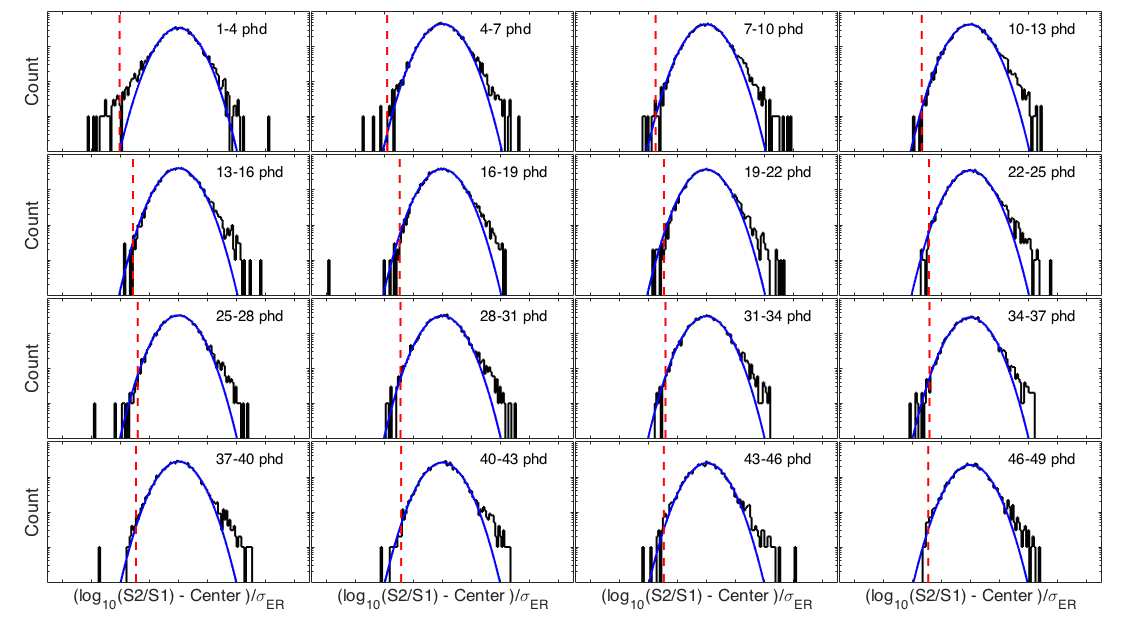
\includegraphics[width=220mm]{fig/Gaussianity/GaussER_all.png}
\caption{Electron recoil population from tritium event about the centroid of the mean in 3 phd bins over the WIMP search region. The red dashed line represents the mean of the NR band in each bin. We observe non Gaussian behavior below three sigma of the ER band and two sigma above. The non Gaussian behavior above the mean of the ER band may be due to the 48\% extraction efficiency.  }
\label{fig:ER-Gauss}
\end{sidewaysfigure}
\twocolumngrid

In Fig. \ref{fig:ER-Gauss} we histogram $\rm log_{10}(S2/S1)$ in bins of S1 with a bin-width of 3 phd. In each bin we show a Gaussian fit to the data after subtracting the centroid and dividing by the Gaussian width. We find that the Gaussian fits describe the data well out to about $2\sigma$ on the upper side and $3\sigma$ on the lower side, beyond which non-Gaussian tails are visible. Only four non-tritium events are expected to be present in these plots out of 180,000 events total, indicating that the small non-Gaussian tails are a genuine feature of ER events in LUX. .... [cite Aaron's thesis ]

In general the width of the ER band should be comprised of three components: the uncertainties on  $\rm n_{\gamma}$ and $\rm n_e$  due to detector resolution ($\rm \sigma(n_{\gamma})$ and $\rm \sigma(n_e)$), and true event-to-event variations in recombination ($\rm \sigma(R)$). $\rm \sigma(n_{\gamma})$ and $\rm \sigma(n_e)$ are responsible for fluctuations in the vertical  and horizontal directions in Fig. \ref{fig:tritium-scatter},  while 
$\rm \sigma(R)$ causes fluctuations along the diagonal lines of constant energy. $\rm \sigma(n_{\gamma})$ and $\rm \sigma(n_e)$ can be measured as a function of energy and are shown in Fig. \ref{fig:recomb-flucs} for LUX tritium data at 180 V/cm\cite{Dobi_Thesis}. Also shown in Fig. \ref{fig:recomb-flucs} is the extracted value of $\rm \sigma(R)$ as a function of energy after controlling for $\rm \sigma(n_{\gamma})$ and $\rm \sigma(n_e)$ by a method described in Ref. \cite{Dobi_Thesis}. 

\begin{figure}[h!]\centering
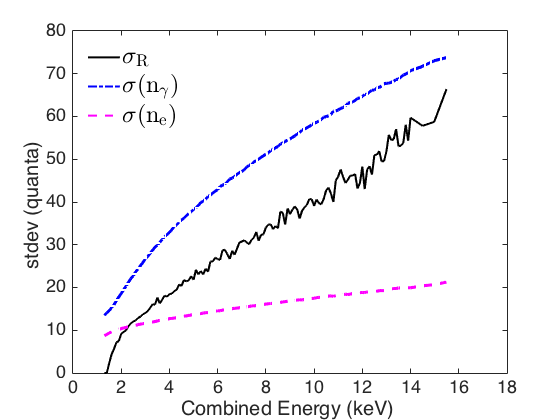
\includegraphics[width=90mm]{fig/recomb_flucs.png}
\caption{Black: recombination fluctuations in LXe measured with LUX tritium data at 180 V/cm. Dot-dash blue: Detector resolution for counting photons. Dashed magenta: Detector resolution for counting electrons.}
\label{fig:recomb-flucs}
\end{figure}

We find that at 180 V/cm in LUX, $\rm \sigma(n_{\gamma})$ is the most important contributor to the ER band width over the entire tritium energy spectrum. Between 2 keVee and 6 keVee, where the WIMP search is most sensitive, $\rm \sigma(n_e)$ and $\rm \sigma(R)$ are of comparable magnitude and secondary importance. We note that an ideal detector would be limited by only $\rm \sigma(R)$.





%Having measured the light and charge yield in-situ we have an understanding of the mean of the electron recoil population for the LUX the WIMP search. To complete the picture we need to understand the variance that lead to the width of the electron recoil band. This is comprise of detector resolution, which is measurable and specific to each detector, and recombination fluctuations. At a given energy the event-to-event standard deviation for the number of recombined ions $\rm \sigma(R)$ is shown in Fig. \ref{fig:recomb-flucs}, extracted using a method outlined in \cite{Dobi_Thesis}. $\rm \sigma(R)$ is a physical property of xenon and produces and irreducible width to the electron recoil band, even with infinite detector resolution. Currently no models exist to predict recombination fluctuations ($\rm \sigma(R)$), thus it is important to measure it in-situ. For the LUX detector conditions we find a linear growth in recombination fluctuations as a function of the number of ions $\rm \sigma(R) = (0.062 \pm 0.005)\cdot N_{ions}$, consistent with the measurement in \cite{Dobi_Thesis}.



%% ER band Gaussianity section. If we want this


%%%%%%%%%%%%%%%%%%%%%%%%%%%%%%%%%%%%%%%%%%%%%%%%%%%%%%%%%%

